\chapter{Uitvoering \& resultaten}
\section{Gebruikte technologi\"en}
Alle programmatie wordt uitgevoerd in Python, een dynamische \textit{high-level} programmeertaal. Python is ontwikkeld met het oog op leesbare en kernachtige code. Het is een van de meest gebruikte talen voor het uitvoeren van wetenschappelijke experimenten, mede dankzij de vele krachtige bibliotheken die beschikbaar zijn. In dit onderzoek worden de volgende Python-bibliotheken gebruikt:

\begin{itemize}
	\item NumPy: voegt ondersteuning toe voor grote, multi-dimensionale arrays en matrices samen met een groot assortiment aan wiskundige functies om deze arrays effici\"ent te  manipuleren. Deze bibliotheek is een onderdeel van de SciPy-stack (Scientific Python).
	\item Theano \cite{theano}:  een bibliotheek die toelaat wiskundige expressies te defini\"eren, optimaliseren en evalueren. De twee belangrijkste troeven van Theano zijn de dynamische generatie van c-code en het transparante gebruik van GPU-acceleratie. Expressies worden symbolisch omgezet en gecompileerd voor een snelle en effici\"ente uitvoering. Ook worden ze geoptimaliseerd  voor gebruik van de GPU.  Hiernaast biedt de bibliotheek ook heel wat functies voor machine learning. 
	\item Lasagne \cite{lasagne}: een lightweight bibliotheek voor het bouwen en trainen van neurale netwerken. Het biedt verschillende veelgebruikte kosten-, regularisatie-, activatie- en leerfuncties aan alsook vele soorten \textit{layers}. Zo gebruikt dit werk de \textit{DenseLayer} voor volledig verbonden lagen en de \textit{Conv2DLayer} voor de tweedimensionale convolutie. Deze bibliotheek bouwt verder op functionaliteit van Theano waardoor neurale netwerken gebouwd met Lasagne ook gebruik kunnen maken van GPU-acceleratie.
	\item Scikit-learn: deze bibliotheek biedt heel wat machine learning functionaliteit aan maar hiervan wordt in dit onderzoek geen gebruik gemaakt. Het pakket binnen scikit-learn dat wel gebruikt wordt, is \textit{metrics}. Deze wordt gebruikt voor de evaluatie van het model. Vanuit de voorspelde en ware labels kunnen we via diverse functies de kwaliteit van de classificatie beschouwen. Dit pakket wordt voornamelijk gebruikt voor het berekenen van de precision en recall, en het opstellen van de confusion matrix. Deze termen worden verklaard in Sectie \ref{sec:pr-conf}.
	\item Scikit-image: is een verzameling beeldverwerkingsalgoritmes. Deze bibliotheek wordt gebruikt voor de data-augmentatie.
	
\end{itemize}
\section{Dataset}
De gebruikte dataset is die van de ``ChaLearn Looking at People Challenge 2014'' \cite{escalera_chalearn_2014}. Uit deze set wordt de derde track gebruikt: ``gesture recognition''. Deze bevat meer dan 14000 gebaren uit een vocabularium van 20 Italiaanse gebaren. Merk op dat het hier niet gaat om een gebarentaal maar om afzonderlijke gebaren uit de Italiaanse cultuur. De verschillende gebaren en hun benamingen zijn te zien in \ref{fig:gebaren}.
\begin{figure}
	\centering
	%	\def\svgscale{0.85}
	\def\svgwidth{\columnwidth}
	\input{figuren/gebaren.pdf_tex}
	\caption{De Italiaanse gebaren gebruikt in de ``ChaLearn Looking At People Challenge 2014, Track 3: gesture spotting''}
	\label{fig:gebaren}
\end{figure}
\npar De gebaren worden uitgevoerd door 27 gebruikers tegen verschillende achtergronden. Er is variatie op vlak van kleding, lichaamsbouw, belichting, gebaaruitvoering. De beelden zijn opgenomen met behulp van een Kinect camera waardoor er vier datastromen zijn: RGB-beeld, dieptebeeld, gebruikersindex en skeletinformatie (Figuur \ref{fig:chalearn-data}).
\begin{figure}
	\centering
	%	\def\svgscale{0.85}
	\def\svgwidth{\columnwidth}
	\input{figuren/chalearn-data.pdf_tex}
	\caption{De vier datastromen beschikbaar in de ``ChaLearn Looking At People Challenge 2014, Track 3: gesture spotting'' dataset}
	\label{fig:chalearn-data}
\end{figure}
\npar Deze dataset werd ook gebruikt in \cite{lionel} waar deze een aantal voorverwerkingsstappen onderging. Deze voorverwerkte dataset is ter beschikking gesteld van dit onderzoek. De voorverwerking probeert de dataset te optimaliseren voor gebarenherkenning. Eerst en vooral worden er vier nieuwe datastromen gecre\"eerd door het uitsnijden van de linker en rechterhand uit zowel diepte- als RGB-beeld. Ook wordt het bovenlichaam ge\"isoleerd om een deel van de achtergrond weg te werken. In totaal zijn er zo zes datastromen beschikbaar. De dataset bestaat uit 10000 ge\"isoleerde gebaren samen met hun correcte klasselabel. Elk beeld bestaat uit 32 frames en heeft een resolutie van 64x64 pixels.

\npar In dit onderzoek wordt de dataset opgedeeld in 60\% training-, 20\% validatie- en 20\% testset.


\section{Onderzoeksopzet}

De experimenten worden uitgevoerd op computers van het Reservoir Lab aan van de vakgroep Elektronica- en Informatiesystemen (ELIS) van de Universiteit Gent. De gebruikte computers hebben een hexacore processor (Intel Core i7-3930K) met kloksnelheid van 3.2 GHz en een NVIDIA Tesla K40c grafische kaart.

\npar In een eerste fase moet er een convolutioneel neuraal netwerk worden opgezet die een aanvaardbare nauwkeurigheid behaald op de gebruikte dataset. Dit model wordt besproken in sectie \ref{sec:basismodel}. De nauwkeurigheden van dit predictief model getraind op alle klassen met alle voorbeelden wordt vervolgens gebruikt als vergelijkingspunt of \textit{baseline} voor de one-shot learning experimenten.

\npar In de volgende stap zal een model, qua architectuur en hyperparameters gelijkend op het basismodel, getraind worden op een deelverzameling van de gebaren. Na deze pre-training kan het model een gebaar bijgeleerd worden en wordt er ge\"experimenteerd met het aantal verschillende samples van het nieuwe gebaar, het aantal lagen dat hertraind worden en met het gebruik van data-augmentatie. De bespreking van deze experimenten gebeurt in sectie \ref{sec:experimenten}.

\section{Basismodel}\label{sec:basismodel}
Alle keuzes omtrent hyperparameters en architectuur zijn experimenteel, op basis van gelijkaardige onderzoeken en naar advies van de begeleiding bepaald. Er zijn vele mogelijke combinaties qua hyperparameters en het is zeer tijdrovend om hierin de meest optimale keuze te maken. Dit is ook niet de essentie van dit onderzoek. Er dient een voldoende goed model opgesteld te worden om vergelijkingen te maken tussen het leren van alle gebaren (basismodel) en het bijleren van een gebaar. 
\subsection{Invoer}
Het beeld van elk gebaar is 64x64 pixels groot en bestaat uit 32 frames. Hieruit worden er 4 frames met volgende indices geselecteerd: 7,13,18 en 25. Er is gekozen om niet van alle input gebruik te maken om een snellere trainingstijd te bekomen zodat er meer experimenten kunenn worden uitgevoerd. In een latere fase of bij verder onderzoek kan het model steeds uitgebreid worden om meer gebruik te maken van spatio-temporele data.
\npar Er wordt enkel gebruik gemaakt van het dieptebeeld, volgens \cite{lionel} en \cite{wu_deep_2014} ligt hierin de nuttigste informatie voor een CNN. Het gebruik van RGB-beeld in combinatie met grijswaardenbeeld voegt meestal weinig toe. Hierin kan dus ook weer rekentijd worden gespaard.
\begin{figure}
	\centering
	%	\def\svgscale{0.85}
	\def\svgwidth{0.5\columnwidth}
	\input{figuren/dataset-input.pdf_tex}
	\caption{De 12 frames gebruikt voor de invoer van het CNN. De frames hebben een resolutie van 64x64 pixels.}
	\label{fig:dataset-input}
\end{figure}
\npar Per voorbeeld zijn er 12 beelden zoals weergegeven in Figuur \ref{fig:dataset-input}. De input van de invoerlaag heeft dus een dimensie van 12x64x64. Merk op dat de beelden van de handen en het volledige bovenlichaam in hetzelfde CNN worden verwerkt. Alle uitgevoerde experimenten hanteren deze invoerdimensie.

\subsection{Architectuur}
\begin{figure}
	\centering
	%	\def\svgscale{0.85}
	\def\svgwidth{\columnwidth}
	\input{figuren/First-model.pdf_tex}
	\caption{Het basismodel bestaande uit een drielagig CNN voor feature-extractie en een drielagig ANN (met softmax uitvoerlaag) voor classificatie}
	\label{fig:model-1}
\end{figure}
Het opgestelde basismodel is weergegeven in figuur \ref{fig:model-1}
Het CNN bestaat uit drie convolutionele en max-pooling lagen. Alle max-pooling gebeurt met vensters van 2x2 zodat het beeld telkens gehalveerd wordt in grootte. De eerste convolutionele laag bevat 8 5x5 filters, de tweede 16 5x5 filters en de laatste 32 4x4 filters.
\npar De output van dit CNN wordt gebruikt als featurevector in een ANN voor classificatie. Het ANN bevat ook drie lagen, de twee verborgen lagen hebben respectievelijk 800 en 100 knopen. Alle verborgen knopen zijn ReLU's en aan de uitgangslaag wordt een softmax gebruikt met 20 units voor de classificatie van de verschillende gebaren.
\begin{table}
	\centering
	%	\vspace{5pt}
	\renewcommand{\arraystretch}{0.8}% 
	\begin{tabular}{ l l }
		\hline
		\textit{Hyperparameter} & \textit{Waarde} \\
		\hline
		\hline
		\textbf{Filters CNN:} & \\
		\quad Laag 1 & 8x(5x5) \\
		\quad Laag 2 & 16x(5x5) \\
		\quad Laag 2 & 32x(4x4) \\
		
		\textbf{Verborgen units ANN:} &\\
		\quad Laag 1 & 800\\
		\quad Laag 2 & 100 \\
		\hline
		Max-pooling vensters & 2x2\\
		Learning rate & $10^{-4}$\\
		Batch grootte & 32\\
		Dropout kans & 0.5\\
		Nesterov momentum & 0.9\\
		\hline
		\textbf{Initialisatie:} & \\
		Gewichten CNN & Glorot initialisatie (uit uniforme verdeling $[-a,a]$)\\
		Bias CNN & 0 \\
		Gewichten ANN & Glorot initialisatie (uit uniforme verdeling $[-a,a]$)\\
		Bias ANN & 0 \\
		\hline
		\textbf{Data-augmentatie:} & \\
		Zoom & [83.33,120] \%, uniforme verdeling \\
		Rotatie & [-2,2]$^{\circ}$, uniforme verdeling\\
		2D translatie & [-2,2] pixels, uniforme verdeling
		
	\end{tabular}	
	\caption{Hyperparameters van het basismodel}\label{tab:hyperparam}
\end{table}
\npar Een samenvatting van alle hyperparameters en gekozen architectuur is te vinden in Tabel \ref{tab:hyperparam}. Voor de regularisatie wordt er gebruik gemaakt van dropout. De gewichten worden ge\"initiaseerd met Glorot gewichten gesampled uit een uniforme verdeling. Deze gewichtsinitialisatie beschreven in \cite{glorot-1} is ontwikkeld voor deep learning methodes en zorgt ervoor dat het signaal tot diep in het netwerk kan reiken. Het is de standaard initialisatie methode van het Lasagne framework.
\npar Er wordt ook aan data-augmentatie gedaan om de prestatie van het predictief model te verbeteren. De gebruikte data-augmentatie bleek bij nader inzien geen zo'n grote impact te hebben door conservatief gekozen parameters zoals weergegeven onderaan Tabel \ref{tab:hyperparam}. In een van de experimenten (sectie \ref{sec:19x1-augm}) worden meer drastische parameters ingezet om het effect van augmentatie nader te onderzoeken.
\subsection{Training}
\npar Mini-batch gradient descent aangevuld met Nesterov Augmented Momentum worden gebruikt als optimalisatie-algoritme. Alle training wordt uitgevoerd op de GPU waardoor we de CPU kunnen gebruiken om de voorbeelden aan te voeren. Dit verloopt als volgt:
\begin{itemize}
	\item een werk-proces selecteert 32 random gekozen klasselabels
	\item per gekozen klasselabel wordt een random voorbeeld van die klasse gekozen uit de trainingset
	\item elk voorbeeld wordt geaugmenteerd met behulp van een transformatiematrix
	\item de voorbeelden worden in een array in het gedeelde geheugen geplaatst en opgehaald voor training van het model
	\item tijdens de training op deze mini-batch wordt de volgende klaargezet
\end{itemize}
Na 250 iteraties, die we verder een epoch zullen noemen, wordt het model ge\"evalueerd met de validatieset. Het minimum van de validatiefout wordt bijgehouden en telkens we een lagere waarde bereiken worden de modelparameters opgeslaan. De training stopt wanneer er na een aantal epochs geen verbetering meer te zien is in de validatiefout.

\subsection{Baseline resultaten}
Om de baseline op te stellen wordt de volledige trainingset gebruikt om de 20 gebaren van de dataset te leren classificeren. Het voorgestelde model convergeert na ongeveer 250 epochs en behaalt een totale nauwkeurigheid van 81,20 \%.

\subsubsection{Precision, recall en confusion}\label{sec:pr-conf}
\begin{figure}
	\centering
	%	\def\svgscale{0.85}
	\def\svgwidth{0.7\columnwidth}
	\input{figuren/prec+recall.pdf_tex}
	\caption{Visualisatie van de betekenis van precision en recall. Links zijn alle relevante elementen te zien die zouden moeten geselecteerd worden. Het omcirkelde gedeelte zijn de effectief geselecteerde elementen of de voorspellingen van het model}
	\label{fig:prec+recall}
\end{figure}

\npar In Figuur \ref{fig:conf-allegebaren} is de genormaliseerde confusion matrix van het basismodel te zien. De mate van verwarring valt best mee, voor alle klassen ligt de waarde op de diagonaal relatief hoog. Een aantal klassen worden wel vaak verward zoals bijvoorbeeld klasse 3 en 9 ($\sim$15 \% van klasse 3 en $\sim$20 \% van klasse 9). Ook klasse 13 en 14 worden ondanks hun relatief hoge ware voorspellingswaarde ook vaak verward ($\sim$7 \% van klasse 13 en $\sim$13 \% van klasse 14)
\npar In Tabel \ref{tab:pr-alle-klassen} zijn alle precision en recall scores van het basismodel opgelijst. Deze scores zullen gebruikt worden als baseline voor de experimenten met het bijleren en one-shotten van een gebaar. Het zijn de waardes die we nastreven bij het hertrainen.
\begin{figure}
	\centering
	
	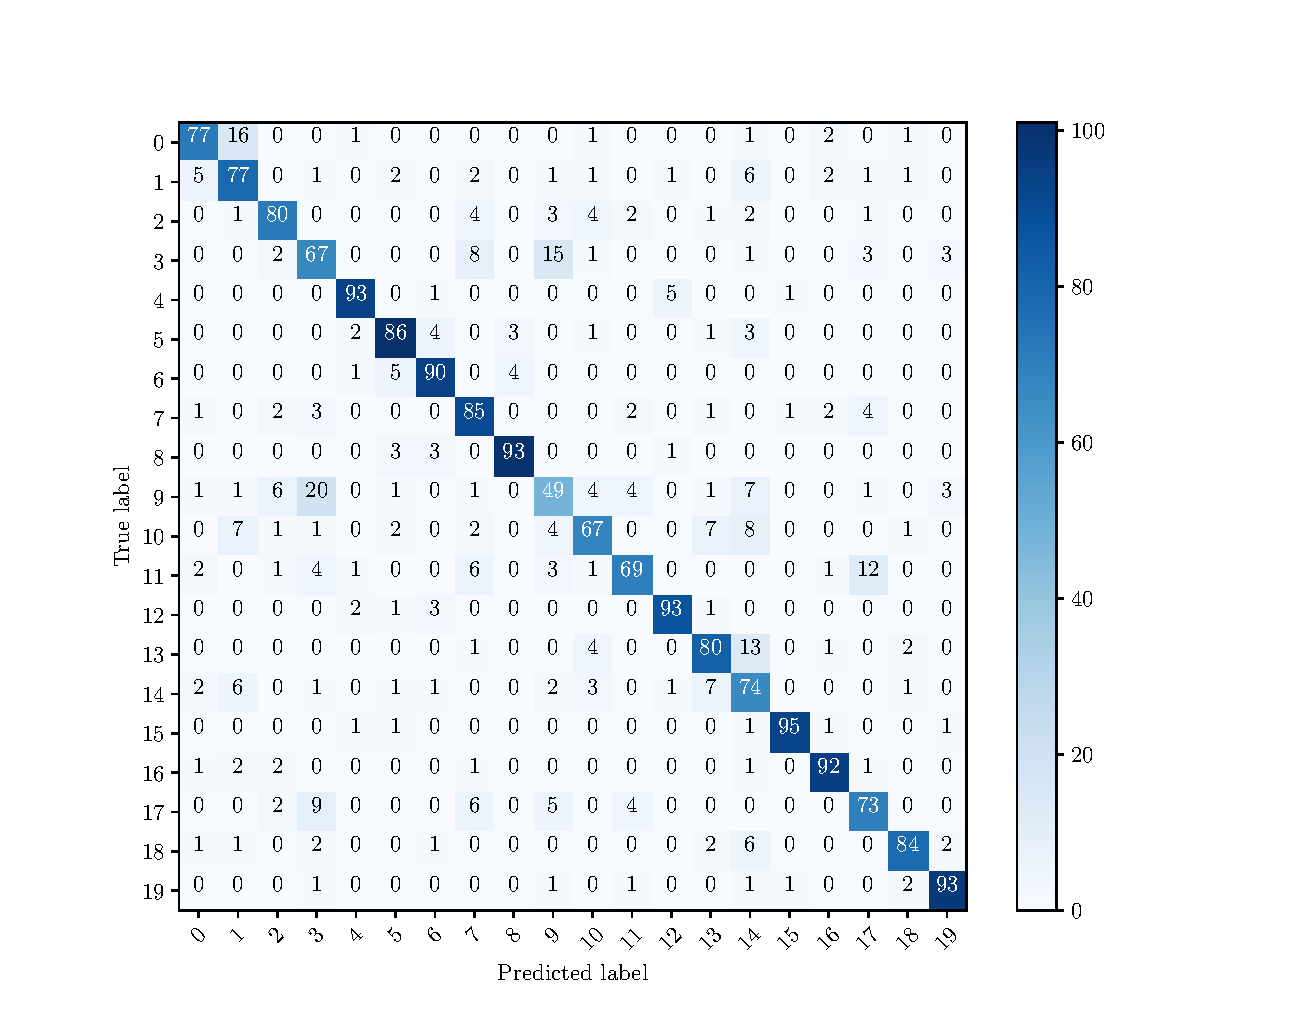
\includegraphics[width=15cm,keepaspectratio]{conf_alle_klassen.pdf}
	\caption{Genormaliseerde confusion matrix van baseline voorspellingen van het basismodel, getraind op alle voorbeelden van alle gebaren }
	\label{fig:conf-allegebaren}

	\vspace{1cm}
	\begin{tabular}{l l}
		\begin{tabular}{l l l}
			\hline
			\textbf{Label} & \textbf{Precision} &
			\textbf{Recall}\\
			\hline
			0 & 84,71 \% & 77,42 \% \\
			1 & 71,17 \% & 77,45 \% \\
			2 & 81,82 \% & 80,00 \% \\
			3 & 62,04 \% & 67,00 \% \\
			4 & 92,15 \% & 93,07 \% \\
			5 & 87,04 \% & 90,38 \% \\
			6 & 84,71 \% & 77,42 \% \\
			7 & 74,59 \% & 85,05 \% \\
			8 & 93,46 \% & 93,46 \% \\
			9 & 58,54 \% & 49,48 \% \\
			\hline
		\end{tabular} & 
		\begin{tabular}{l l l}
			\hline
			\textbf{Label} & \textbf{Precision} &
			\textbf{Recall}\\
			\hline
			10 & 77,27 \% & 67,33 \% \\
			11 & 84,33 \% & 69,31 \% \\
			12 & 91,57 \% & 92,55 \% \\
			13 & 80,39 \% & 79,61 \% \\
			14 & 56,41 \% & 74,16 \% \\
			\textbf{15} & \textbf{96,88} \% & \textbf{94,90} \% \\
			16 & 91,35 \% & 92,23 \% \\
			17 & 75,27 \% & 72,92 \% \\
			18 & 90,69 \% & 83,87 \% \\
			19 & 91,51 \% & 93,27 \% \\
			\hline
		\end{tabular}	
	\end{tabular}
	\captionof{table}{Precision en recall voor de voorspellingen van het basismodel getraind op alle voorbeelden van alle gebaren.}
	\label{tab:pr-alle-klassen}
\end{figure}


\section{Een gebaar bijleren}\label{sec:experimenten}

\subsection{Softmax 20}

De eerste experimenten rond het bijleren van een gebaar worden uitgevoerd op een model volledig gelijk aan het basismodel (zoals afgebeeld in Figuur \ref{fig:model-1}). Eerst wordt het model getraind met een trainingset van 19 gebaren. Als het model geconvergeerd is en genoeg geregulariseerd, zou het een aantal algemene features van een nieuw gebaar moeten herkennen.

\npar De pretraining gebeurt op een softmax van 20 units, een unit wordt dus niet gebruikt. Deze opstelling is natuurlijk niet erg bruikbaar om een dynamisch uitbreidbaar herkenningssysteem te maken maar is wel een goede eerste test van het potenti\"eel van het model.

\npar Door het model te hertrainen met de trainset van 19 gebaren aangevuld met een aantal samples van het nieuwe gebaar leren we het model ook op deze klasse te activeren. Om de hyperparameters van het model te optimaliseren wordt het na elke epoch ge\"evalueerd met de volledige validatieset. Deze bevat alle voorbeelden van het nieuwe gebaar zodat er goed kan gelet worden op overfitting.

\npar Een finale evaluatie wordt gemaakt met alle voorbeelden uit de testset. 

\subsubsection{Invloed aantal samples}
Eerst en vooral wordt het aantal samples gevari\"eerd. Het model wordt getraind met 200, 100, 50, 25, 10, 5, 4, 3, 2 voorbeelden en ten slotte wordt er 1 voorbeeld gebruikt voor een poging tot one-shot learning.

\npar In figuur \ref{fig:naive-model} zijn twee plots te zien van het bijleren van gebaar nummer 15: "non ce ne piu". De precision en recall scores van twee experimenten zijn er te zien. Het basismodel getraind op alle voorbeelden behaalde een 96.88\% precision en 94.90\% recall score op dit gebaar. De hoogste scores van alle gebaren. Enerzijds zou dit gebaar dus makkelijk moeten aan te leren zijn aangezien het heel nauwkeurig voorspeld wordt. Anderzijds kan het model zich niet meer beroepen op de features geleerd uit dit gebaar.
\npar Het is opvallend dat de precision scores voor beide modellen heel dicht liggen bij de baseline. Het model is dus redelijk zeker dat het om het nieuwe gebaar gaat als het dit gebaar herkent. Bij het hertrainen van de twee laatste lagen met twee voorbeelden gaat de precisie zelfs eventjes boven die van de baseline.

\npar De recall score volgt niet dezelfde lijn als die van de precision. Hier zien we duidelijk dat de recall bij gebruik van weinig samples heel laag ligt. De stijlste klimming bij het model waar enkel de softmax wordt hertraind (Figuur \ref{fig:naive-oneshot-gebaar15}) zien we tot aan het gebruik van 5 samples. Bij het hertrainen van twee lagen (Figuur \ref{fig:naive-oneshot-gebaar15-2lagen}) loopt deze stijging door tot 10 samples. Er worden meer parameters geoptimaliseerd bij de training van het tweede model en meer parameters betekent meer voorbeelden. Dit model maakt dus beter gebruik van het grotere aantal samples.

\npar Het model

\begin{figure}
	\begin{subfigure}[b]{\textwidth}
		\centering
		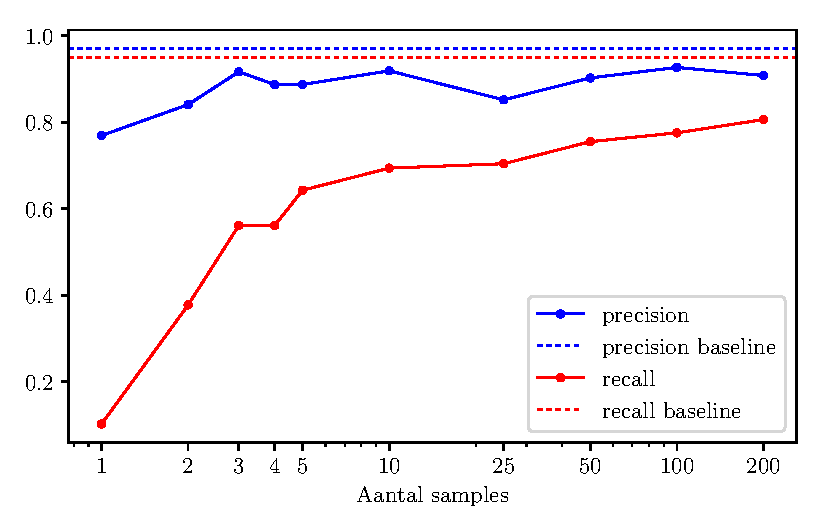
\includegraphics[width=10cm,keepaspectratio]{naive-oneshot-gebaar15.pdf}
		\subcaption{Hertrainen softmax laag}\label{fig:naive-oneshot-gebaar15}
	\end{subfigure}%
	\par
	\begin{subfigure}[b]{\textwidth}
		\centering
		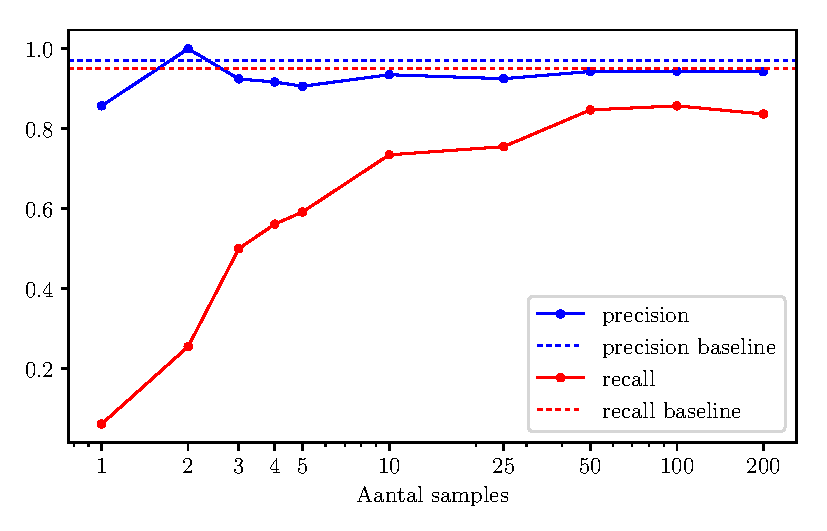
\includegraphics[width=10cm,keepaspectratio]{naive-oneshot-gebaar15-2lagen.pdf}
		\subcaption{Hertrainen dense100 en softmax laag}		\label{fig:naive-oneshot-gebaar15-2lagen}
	\end{subfigure}
	\caption{Precision en recall voor de classificatie van gebaar 15 met het softmax20 model in functie van het aantal gebruikte samples voor bijleren. De streepjeslijn geeft de baseline weer van het model getrained op alle voorbeelden.}\label{fig:naive-model}
\end{figure}

\subsection{Softmax 19 + 1}
\subsubsection{Invloed aantal samples}
\subsubsection{Invloed data-augmentatie}\label{sec:19x1-augm}

\subsection{Softmax 18 + 2}